\begin{figure}
  \centering
  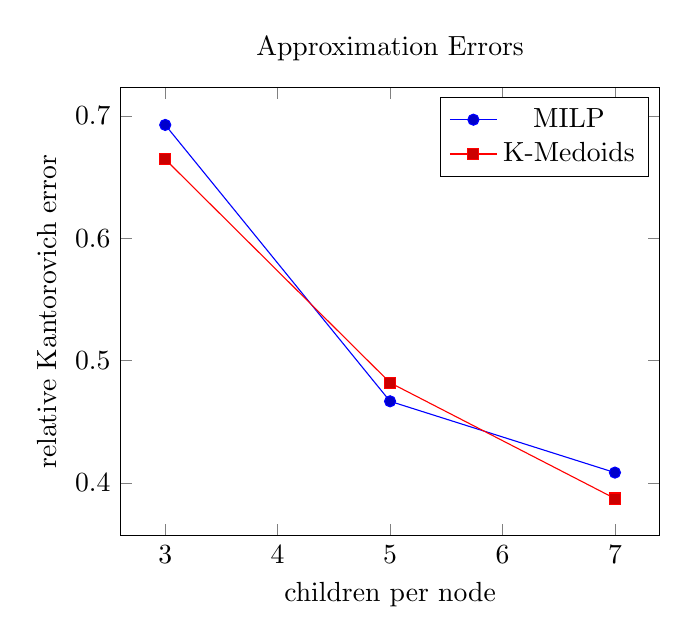
\begin{tikzpicture}
    \begin{axis}% Errors over number of children
      [
      title=Approximation Errors,
      legend entries={MILP,K-Medoids},
      xlabel=children per node,
      ylabel=relative Kantorovich error
      ]
      \addplot coordinates { % testscen=1000
        (3, 0.6927)
        (5, 0.4667)
        (7, 0.4084)
      };
      \addplot coordinates { % testscen=3000
        (3, 0.6646)
        (5, 0.4819)
        (7, 0.3872)
      };
    \end{axis}
  \end{tikzpicture}
    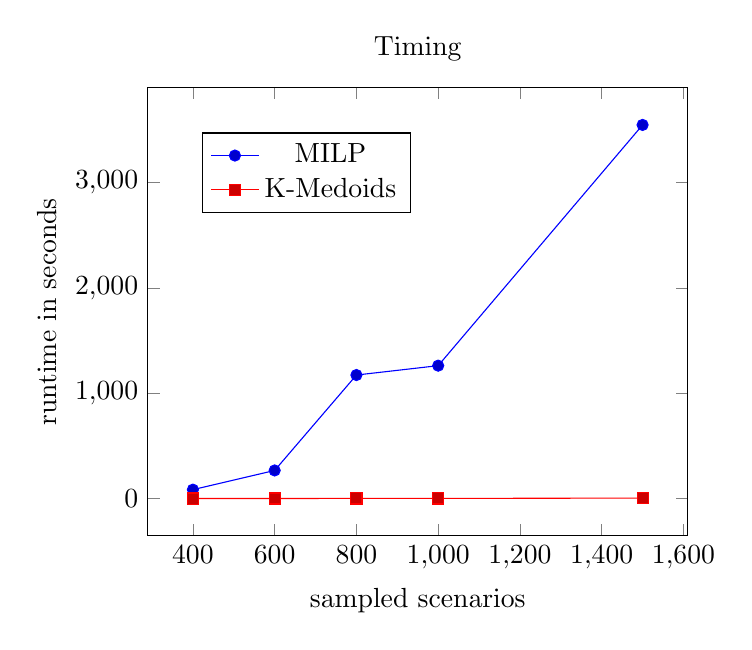
\begin{tikzpicture}
    \begin{axis}% Timing, nchildren=3,nstages=3
      [
      title=Timing,
      legend entries={MILP,K-Medoids},
      xlabel=sampled scenarios,
      ylabel=runtime in seconds,
      legend style={at={(0.1,0.9)},anchor=north west}
      ]
      %\addplot coordinates { % testscen=3000, time in seconds
      %  (3, 32.2653)
      %  (5, 39.2829)
      %  (7, 71.1328)
      %};
      \addplot coordinates{ % MILP
        (400, 85.1)
        (600, 267.4)
        (800, 1172.9)
        (1000, 1261.9)
        (1500, 3546.5)
      };
      \addplot coordinates { % K-medoids
        (400, 0.9120)
        (600, 1.3498)
        (800, 1.9716)
        (1000,1.7055)
        (1500,5.3441)
      };
    \end{axis}
  \end{tikzpicture}
  \caption{Comparison of the stage-wise MILP and K-Medoids algorithm.
    The figure above plots the relative error in the Kantorovich distance of the scenario trees generated by the stage-wise MILP algorithm and the tree-K-Medoids algorithm for different filtration trees.
    Both algorithms achieve very similar qualities of approximation.
    The plot below shows the run time of the algorithms for different sizes of input data.
    The K-Medoids algorithm proves to be very scalable.
  }
  \label{fig:compare-milp-kmedoids}
\end{figure}
%%% Local Variables:
%%% mode: latex
%%% TeX-master: "da"
%%% End:
